\documentclass{article}
\usepackage{tikz}
\definecolor{darkgreen}{RGB}{0,192,0}
\title{Cartesian closed categories and the price of eggs}
\author{Jane Doe}
\date{September 1994}
\begin{document}

	\usetikzlibrary{arrows.meta}
	\tikzset{>={Latex[width=3mm,length=3mm]}}

	\begin{figure}
		% bezier curve diagram
		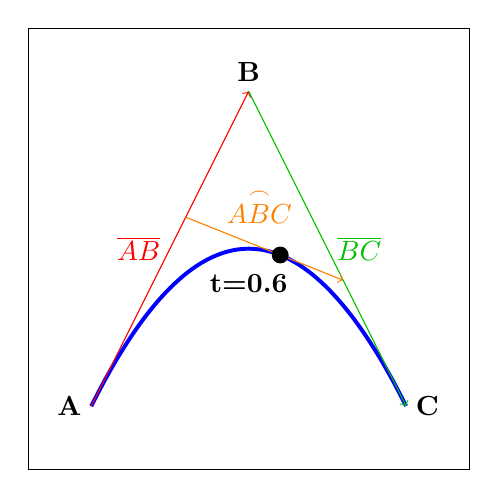
\begin{tikzpicture}[x=4cm,y=4cm]
			% border
			\draw (-0.2,-0.2) -- (1.2,-0.2) -- (1.2,1.2) -- (-0.2,1.2) -- (-0.2,-0.2);
			% 1d quadratic bezier curve with control points 0,1,0
			\draw[scale=1,domain=0:1,smooth,variable=\x,blue,line width=0.5mm] plot ({\x},{2*\x-2*\x*\x});		
			% control polygon / labels
			\draw[red,->]       (0.0,0.0) -- (0.5,1.0);
			\draw[darkgreen,->] (0.5,1.0) -- (1.0,0.0);
			\draw[red]          (0.25,0.5) node[anchor=east] {$\overline{AB}$};
			\draw[darkgreen]    (0.75,0.5) node[anchor=west] {$\overline{BC}$};
			% control point labels
			\draw (0.0,0.0) node[anchor=east]  {\bf{A}};
			\draw (0.5,1.0) node[anchor=south] {\bf{B}};
			\draw (1.0,0.0) node[anchor=west]  {\bf{C}};
			% draw a line from AB->AC for time = 0.75
			\draw[orange,->] (0.3,0.6) -- (0.8,0.4);
			\draw[orange] (0.40,0.55) node[anchor=south west] {$\stackrel{\frown}{ABC}$};
			% draw the point at t=0.6 and label underneath the curve
			\draw[black,fill=black] (0.6,0.48) circle (1mm);
			\draw[black] (0.5,0.45) node[anchor=north] {\bf{t}=0.6};
		\end{tikzpicture}
		% bilinear diagram
		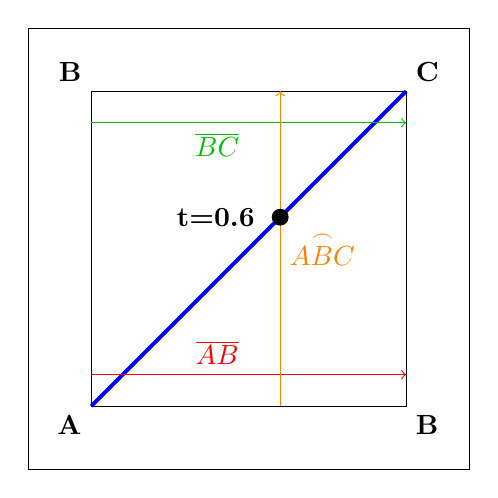
\begin{tikzpicture}[x=4cm,y=4cm]
	    	% border
	    	\draw (-0.2,-0.2) -- (1.2,-0.2) -- (1.2,1.2) -- (-0.2,1.2) -- (-0.2,-0.2);
	    	% box
	    	\draw (0,0) -- (1,0) -- (1,1) -- (0,1) -- (0,0);
	    	% representative line for where the quadratic bezier curve lives
	    	\draw[blue,line width=0.5mm] (0,0) -- (1,1);		
	    	% corner labels
	    	\draw (0,0) node[anchor=north east] {\bf{A}};
	    	\draw (1,0) node[anchor=north west] {\bf{B}};    	
	    	\draw (0,1) node[anchor=south east] {\bf{B}};
	    	\draw (1,1) node[anchor=south west] {\bf{C}};    	
	    	% x axis interpolation
	    	\draw[red,->]       (0.0,0.1) -- (1.0,0.1);
	    	\draw[red]          (0.4,0.1) node[anchor=south] {$\overline{AB}$};
	    	\draw[darkgreen,->] (0.0,0.9) -- (1.0,0.9);
	    	\draw[darkgreen]    (0.4,0.9) node[anchor=north] {$\overline{BC}$};
	    	% y axis interpolation
	    	\draw[orange,->]    (0.6,0.0) -- (0.6,1.0);
	    	\draw[orange]    	(0.6,0.5) node[anchor=west] {$\stackrel{\frown}{ABC}$};
	    	% draw the point at t=0.6 and label for it
	    	\draw[black,fill=black] (0.6,0.6) circle (1mm);
	    	\draw[black] (0.55,0.6) node[anchor=east] {\bf{t}=0.6};
		\end{tikzpicture}	
		\caption{Left: A quadratic Bezier curve evaluated at {\bf{t}}=0.6 for control points A,B,C using the De Casteljeau algorithm.  Right: The De Casteljeau algorithm using bilinear interpolation.  Note that in this case, the X axis is evaluated before the Y, but the Y axis could be evaluated before the X for the same results.}
	\end{figure}			

\end{document}